% =========================================================================
\chapter{Extreme value theory (EVT)}
\label{ch:evt}
% =========================================================================

\section{Why a special theory for extremes}
Ordinary statistics (mean, standard deviation, normal curve) describe the \emph{typical} values, where almost all data
lie. The \textbf{tail}, the far end with the rare extremes, has very few points, and a curve fitted to all the data
usually gets the tail wrong. \textbf{Extreme value theory} is the branch of statistics that models only the tail.

\begin{keyidea}[In one line]
Model the tail, not the average.
\end{keyidea}

\section{Two ways to do EVT}
\begin{center}
\footnotesize
\begin{tabular}{p{3.2cm}p{5.2cm}p{2.6cm}c}
\toprule
\textbf{Approach} & \textbf{Data it uses} & \textbf{Distribution} & \textbf{Used here?}\\
\midrule
Block maxima & the single largest value of each block (e.g.\ hottest day of each year) & GEV (generalised extreme
  value) & No\\
\textbf{Peaks over threshold} & \textbf{every value above a high threshold} & \textbf{GPD (generalised Pareto)} &
  \textbf{Yes}\\
\bottomrule
\end{tabular}
\end{center}
Peaks over threshold uses every extreme day, not just one per year, so it gets more information from the same record.

\section{Threshold, exceedance and excess}
\begin{itemize}
  \item \textbf{Threshold $u$:} the 99th percentile of the cell and season (Chapter~\ref{ch:extreme}). \emph{We chose}
        this value; the theory only asks that it be high.
  \item \textbf{Exceedance:} a day above $u$, i.e.\ an extreme day.
  \item \textbf{Excess:} how far above, $T^{\max}-u$, in $^\circ$C.
\end{itemize}

\section{Standardising: the severity $z$}
An excess of 2\,$^\circ$C is huge in a calm valley cell and ordinary in a variable mountain cell. So each excess is
divided by $s$, the cell's own day-to-day spread (the standard deviation of its daily temperature anomaly in that
season):
\[
  z=\frac{T^{\max}-u}{s}.
\]
Now all 529 cells are on one scale, and one curve per season can be fitted to all of them together. $z$ is the
\textbf{severity} of an extreme day: 0 means just over the threshold, larger means more severe.

\section{The generalised Pareto distribution (GPD)}
\begin{keyidea}[The theorem behind EVT (Pickands--Balkema--de Haan)]
Whatever the original data look like, the excesses above a high enough threshold follow (approximately) a
\textbf{generalised Pareto distribution}.
\end{keyidea}

The chance that the severity is larger than $z$ is
\[
  P(Z>z)=\Big(1+\frac{\xi z}{\sigma}\Big)^{-1/\xi},\qquad z\ge0,
\]
with two numbers to fit: the \textbf{scale} $\sigma$ (the typical size of an excess) and the \textbf{shape} $\xi$
(``xi''), which decides the kind of tail.

\begin{figure}[H]
\centering
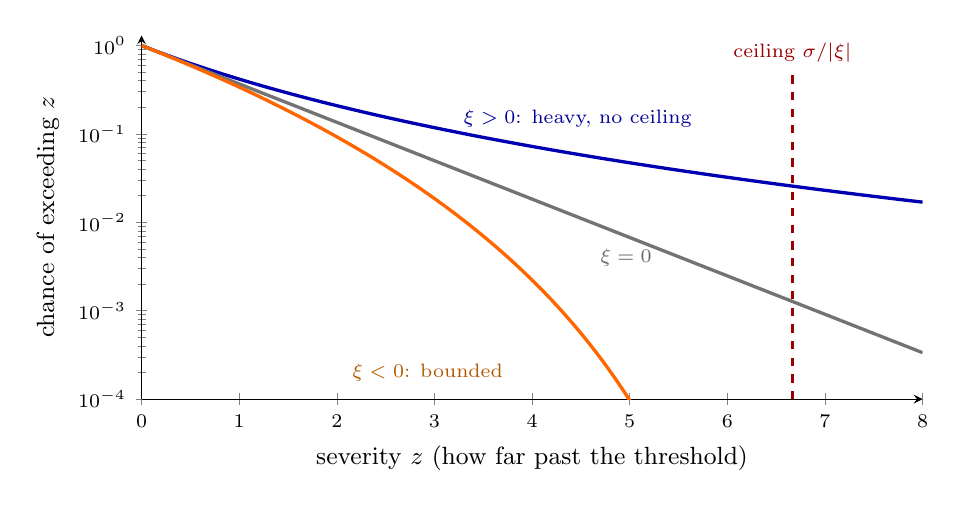
\begin{tikzpicture}
\begin{semilogyaxis}[width=11.5cm,height=6.2cm,axis lines=left,xmin=0,xmax=8,ymin=1e-4,ymax=1.3,
  xlabel={severity $z$ (how far past the threshold)},ylabel={chance of exceeding $z$},
  xlabel style={font=\small},ylabel style={font=\small},tick label style={font=\scriptsize},samples=300]
\addplot[very thick,blue!70!black,domain=0:8] {(1+0.3*x)^(-1/0.3)};
\addplot[very thick,black!55,domain=0:8] {exp(-x)};
\addplot[very thick,orange!80!red,domain=0:6.6] {(1-0.15*x)^(1/0.15)};
\draw[dashed,thick,red!60!black] (axis cs:6.667,1e-4) -- (axis cs:6.667,0.5);
\node[font=\scriptsize,red!60!black,anchor=south] at (axis cs:6.667,0.5) {ceiling $\sigma/|\xi|$};
\node[font=\scriptsize,blue!60!black,anchor=west] at (axis cs:3.2,0.15) {$\xi>0$: heavy, no ceiling};
\node[font=\scriptsize,black!60,anchor=west] at (axis cs:4.6,0.004) {$\xi=0$};
\node[font=\scriptsize,orange!70!black,anchor=east] at (axis cs:3.8,2e-4) {$\xi<0$: bounded};
\end{semilogyaxis}
\end{tikzpicture}
\caption{The three kinds of GPD tail ($\sigma=1$). With $\xi<0$ the chance drops to zero at a finite ceiling.}
\end{figure}

\begin{center}
\footnotesize
\begin{tabular}{lll}
\toprule
\textbf{Shape} & \textbf{Tail} & \textbf{Meaning}\\
\midrule
$\xi>0$ & heavy & no upper limit; huge values possible (floods, insurance losses)\\
$\xi=0$ & exponential & falls off steadily\\
$\xi<0$ & bounded & a \textbf{ceiling} at $z^*=\sigma/|\xi|$; values cannot go beyond it\\
\bottomrule
\end{tabular}
\end{center}
For temperature, physics suggests a ceiling, so we expect $\xi<0$.

\section{How the GPD was fitted}
\begin{itemize}
  \item \textbf{Data:} the standardised severities $z$ of all extreme days of 1981--2010; one fit per season (and one
        for the whole year), pooling all 529 cells.
  \item \textbf{Method: maximum likelihood.} Choose $\sigma$ and $\xi$ that make the observed severities most probable
        (\texttt{scipy.stats.genpareto.fit}, with the curve starting at 0).
  \item \textbf{Uncertainty: bootstrap.} Refit 100 times on resampled data and take the middle 95\% of the shapes as the
        95\% range. Whole days are resampled together, because an extreme usually hits many cells on the same day (on
        6 October 1983, 522 of the 529 cells were extreme).
  \item \textbf{Checks:} refitting only on the upper part of the tail gave similar shapes (threshold stability), and a
        plot of fitted against real values agreed.
\end{itemize}

\section{What the fit found}
\begin{center}
\footnotesize
\begin{tabular}{lccc}
\toprule
\textbf{Season} & \textbf{$\xi$ before standardising} & \textbf{$\xi$ after} & \textbf{95\% range (after)}\\
\midrule
Whole year & $-0.153$ & $-0.152$ & $-0.196$ to $-0.113$\\
Monsoon & $-0.128$ & $-0.115$ & $-0.185$ to $-0.040$\\
Pre-monsoon & $-0.165$ & $-0.141$ & $-0.241$ to $-0.072$\\
Winter & $-0.074$ & $-0.096$ & $-0.176$ to $-0.032$\\
Post-monsoon & $+0.262$ & $+0.070$ & $-0.177$ to $+0.231$\\
\bottomrule
\end{tabular}
\end{center}
\begin{itemize}
  \item Every season is negative or about zero: \textbf{heat in Himachal has a ceiling}.
  \item Post-monsoon looked heavy-tailed ($+0.26$) before standardising. That was an artefact of mixing cells with
        different variability; after standardising it is $+0.07$ and its range includes 0.
\end{itemize}

\section{Tail position $q$}
The fitted GPD turns a severity $z$ into a \textbf{tail position} $q=F(z)$, a number between 0 and 1, where $F$ is the
GPD's cumulative probability. $q=0.9$ means ``more severe than 90\% of the extreme days of that season''. The reverse,
turning a $q$ back into a severity, is $z=F^{-1}(q)$, the GPD's \emph{quantile function}. Drawing random $q$'s and
turning them into $z$'s this way is called \textbf{inverse-transform sampling}.

\section{EVT tail focus: where the 60\% comes from}
For every 100 days to be added, 50 get a $q$ drawn evenly between 0 and 1 (``anywhere in the tail'') and 50 get a $q$
drawn evenly between 0.8 and 1 (``only the top fifth''):
\[
  q\sim0.5\,\mathcal{U}(0,1)+0.5\,\mathcal{U}(0.8,1),\qquad
  P(q\ge0.8)=0.5\times0.2+0.5\times1=0.6 .
\]

\begin{figure}[H]
\centering
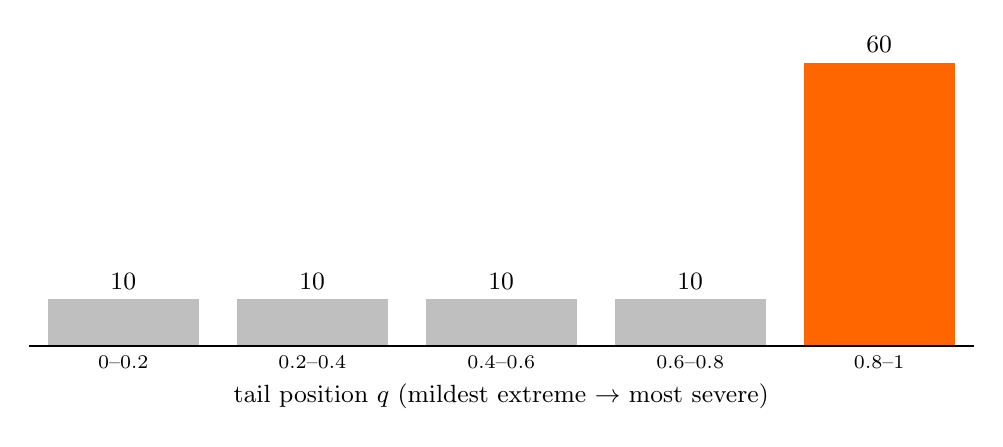
\begin{tikzpicture}[x=2.4cm,y=0.06cm]
\foreach \i/\v/\c in {0/10/black!25,1/10/black!25,2/10/black!25,3/10/black!25,4/60/orange!80!red}{
  \fill[\c] (\i+0.1,0) rectangle (\i+0.9,\v);
  \node[font=\small,anchor=south] at (\i+0.5,\v) {\v};}
\draw[thick] (0,0) -- (5,0);
\foreach \i/\l in {0/0--0.2,1/0.2--0.4,2/0.4--0.6,3/0.6--0.8,4/0.8--1}
  \node[font=\scriptsize,anchor=north] at (\i+0.5,0) {\l};
\node[font=\small,anchor=north] at (2.5,-6) {tail position $q$ (mildest extreme $\rightarrow$ most severe)};
\end{tikzpicture}
\caption{Of 100 added days, 10 fall in each of the four lower fifths (all from the ``anywhere'' half) and 60 in the top
fifth (10 + 50).}
\end{figure}

\begin{itemize}
  \item \textbf{Why not all 100 at the top?} Then the mild extremes would get no new examples and the model could get
        worse at them. Keeping half ``anywhere'' gives every part of the tail some new days.
  \item \textbf{Cap:} each $z$ is limited to the ceiling $\sigma/|\xi|$ and to 1.5 times the hottest real extreme of
        that season, so no added day is hotter than possible.
  \item \textbf{Plain (no EVT):} the comparison version simply uses severities as they occur in the real extremes.
\end{itemize}

\section{What EVT did not do in this project}
No block maxima, no GEV distribution, no return levels (``1-in-100-year heat''), and EVT was not built into the
training of the generators. It was used to \emph{rank} severity, to \emph{choose} the severities of added days, and to
\emph{cap} them.

\begin{sayit}
``Extreme value theory models only the tail. Above a high threshold, how far days go past it follows a generalised
Pareto distribution. I fitted one per season: the shape is negative, so heat has a ceiling. I then used it to put 60\%
of the added days in the rarest 20\% of the tail, and never above the ceiling.''
\end{sayit}
